\documentclass[../main.tex]{subfiles}

\begin{document}
\begin{CJK*}{UTF8}{gbsn}

\section*{Exercice 1bc}
Produisez un graphique de Kaplan-Meier utilisant l'échantillon entier,
le groupe de \texttt{trt = 0} et le groupe de \texttt{trt = 1} 
pour le temps jusqu'à devenir aveugle.
Décrivez le courbe de survie dans vos mots.

\paragraph{Solution}

Nous avons obtenu un graphique montrant la probabilité de survie pour 
l'ensemble de l'échantillon depuis le début du traitement jusqu'à la cécité 
(définie comme une baisse de l'acuité visuelle à $\frac{5}{200}$). 
La courbe commence à $1$ (soit une probabilité de survie de $100 \%$) et diminue progressivement.
Par conséquent, il y a plus de risques de devenir aveugle au fil du temps.
Sur l'axe des abscisses, le temps est indiqué en jours.
L'axe des ordonnées montre la proportion de patients 
qui n'ont pas encore diagnostiqué de cécité à un moment donné.
Le graphique en R comporte trois courbes qui représentent 
la probabilité de survie de l'échantillon entier (représenté en noir), 
du groupe non traité (représenté en rouge, \texttt{trt = 0}) 
et du groupe traité (représenté en bleu, \texttt{trt = 1}). 

\begin{lstlisting}
#Kaplan-Meier 
result.km <- survfit(Surv(time, status) ~ 1, conf.type="log-log")
plot(result.km, xlab = "Jours", ylab = "Probabilite de Survie", main = "Kaplan-Meier")
result.kmtrt0 <- survfit(Surv(time[trt == 0], status[trt == 0]) ~ 1, conf.type="log-log")
par(new=TRUE)
plot(result.kmtrt0, xlab = "Jours", ylab = "Probabilite de Survie", main = "Kaplan-Meier", col = "red")
result.kmtrt1 <- survfit(Surv(time[trt == 1], status[trt == 1]) ~ 1, conf.type="log-log")
par(new=TRUE)
plot(result.kmtrt1, xlab = "Jours", ylab = "Probabilite de Survie", main = "Kaplan-Meier", col = "blue")
legend("topright", legend=c("totale","trt = 0", "trt = 1"), col=c("black","red", "blue"), lty=1:5, cex=0.8)
#abline ( v = 43.7 , col = 'red' , lty =2)
\end{lstlisting}

Le plot est :

\begin{figure}[H]
  \centering
  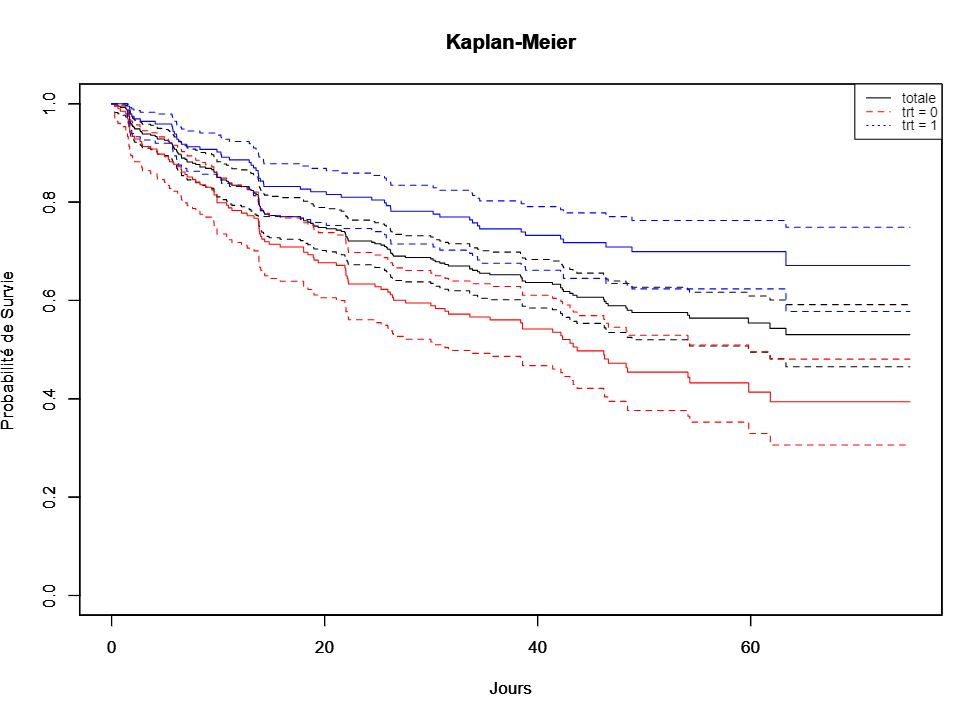
\includegraphics[width=0.8\textwidth]{1BC.JPG}
  \label{fig:mesh1}
\end{figure}

Le graphique montre que la courbe de survie du groupe traité est 
plus élevée que celle du groupe non traité à la plupart des moments, 
ce qui suggère que le traitement puisse aider à retarder l'apparition de la cécité. ////

\end{CJK*}
\end{document}

\end{CJK*}
\end{document}